\documentclass[12pt]{article}
\usepackage{amsmath,amsfonts,amssymb,amsthm}
\usepackage[pdftex]{graphicx}
\pagestyle{plain}
\title{Back Propogation Project}
\author{Daniel Haskin}
\begin{document}
\maketitle
\section{Introduction}
Backpropogation is a method by which we may train an artificial nueral network
to classify data more and more accurately. In this project, I implement the
backpropogation algorithm, and use it to find out what choices of parameters
yield the best predictive accuracy using the Iris and Vowel datasets.
\section{Methods}
\subsection{Basic Implemented Functionality}
In my implementation of the backpropogation algorithm, I implemented
the following functionality:
\begin{enumerate}
\item The neural network updates its weights incrementally
\item Ability to add arbitrarily large layers to the network using the
    \texttt{--add-layer} option
\item Random weight initialization using a standard Gaussian distribution
\item Random shuffling (randomization) of the data at the beginning of each
    training epoch.
\item Optional momentum term via the \texttt{-m} option.
\end{enumerate}
\subsection{Stopping Criteria}
As to stopping criteria, I decided to look at the mean squared error (MSE) at
each epoch, or specifically its improvement. I kept track of the MSE on the
current epoch and also the MSE for the previous epoch is below threshold (chosen
as $0.001$), multiplied by the learning rate, I decided to stop. I included the
learning rate in the decision, reasoning that if the learning rate was small,
improvement over an epoch may be small enough to be under threshhold, yet very
far away from acheiving a minima with respect to MSE.
\section{Iris Problem}
\subsection{Choosing A Learning Rate}

As per the project specifications, I looked at several different learning rates
to determine the best learning rate for the iris dataset. I tried various
learning rates using a single layer of 8 nodes. My findings are summarized in
    figures \ref{fig:learning_rate_accuracy} and
\ref{fig:learning_rate_epochs}.
\begin{figure}[!ht]
    \begin{center}
        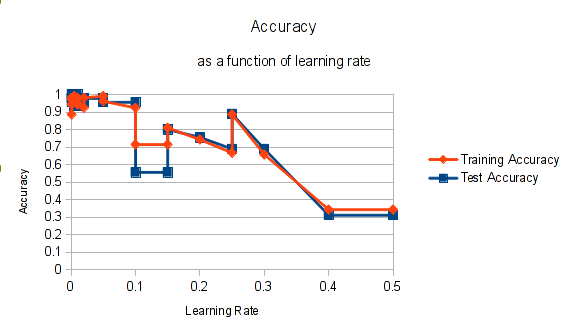
\includegraphics[width=0.75\textwidth]{Iris-LearningRate-Accuracy}
    \end{center}
    \caption{Accuracy as a function of learning rate.}
  \label{fig:learning_rate_accuracy}
\end{figure}

\begin{figure}[!ht]
    \begin{center}
        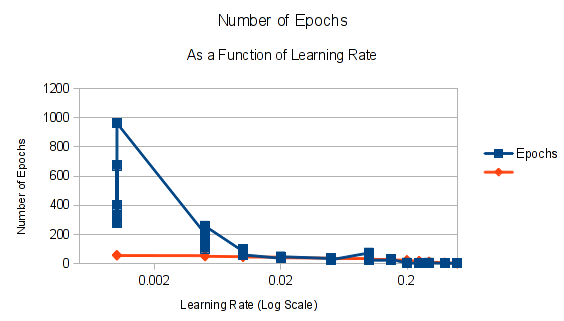
\includegraphics[width=0.75\textwidth]{Iris-LearningRate-Epochs}
    \end{center}
    \caption{Number of epochs required to train as a function of learning rate.
    Note the log scale of the x-axis.}
  \label{fig:learning_rate_epochs}
\end{figure}

Looking at these graphs, it is clear that there is an accuracy-epoch trade-off.
When the learning rate is very small, the accuracy never seems to get worse,
though it seems there is diminishing return on accuracy as one decreases the
learning rate. However, for small learning rates, the number of epochs required
to train a dataset explodes as the learning rate increases, even when shown on
a log scale.

Looking at both graphs, it seems that $0.05$  seems like a good choice. It gets
very high accuracy, yet still has a manageable number of epochs before the
stopping criteria is satisfied.
\subsection{Node Count}
I graphed accuracy against number of nodes in a single hidden layer. I also
graphed number of epochs needed to train the model before stopping
criteria was reached. I graphed data points, for 1, 2, 4, 8, 16, and 32 nodes.

Looking at figures \ref{fig:node_count_accuracy} and
\ref{fig:node_count_epochs}, we can see that both the accuracy and number
of epochs needed start to be fairly constant after $8$ nodes. This may be
because that is $2n$, or twice the number of inputs (there are 4 inputs in the
Iris dataset). This makes sense because in a linear space, that is the number
of hyperplanes needed to create a hyper cube (i.e., a hypercube in
$n$-dimentional space has $2n$ sides).

\begin{figure}[!ht]
    \begin{center}
        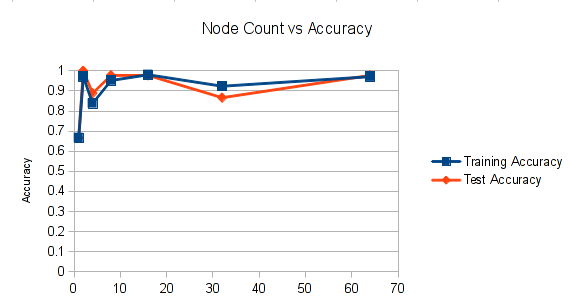
\includegraphics[width=0.75\textwidth]{Iris-NodeCount-Accuracy}
    \end{center}
    \caption{Accuracy graphed as a functions of the number of nodes used in a
    single hidden layer.}
  \label{fig:node_count_accuracy}
\end{figure}
\begin{figure}[!ht]
    \begin{center}
        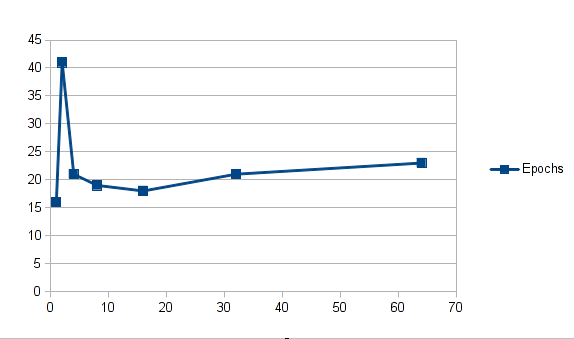
\includegraphics[width=0.75\textwidth]{Iris-NodeCount-Epochs}
    \end{center}
    \caption{Number of Epochs needed to train graphed as a function of the
    number of nodes used in a single hidden layer.}
  \label{fig:node_count_epochs}
\end{figure}
\end{document}
